\section{Force estimation}
In order to have a representation of the reaction force on the EndoWrist, estimation is needed.
Because of the reasons mentioned in Section \ref{sec:system_overview}, the force cannot be measured using sensors and thus have to rely on mathematical models as functions of torque measurements.


\subsection{Mathematical model}
The main challenge faced in making a model lies in the fact that the pulley system on the EndoWrist is nonlinear, and thus its full dynamics cannot be modeled in a straightforward manner. 
In other words, to have an accurate representation of Cartesian force a higher order model is required.

Another method of tackling this problem is to create multiple mathematical models pertaining to forces output by actions performed with the EndoWrist.
In this manner, the feedback vector is transformed from Cartesian space to a task space in which the chosen actions form a basis.
Each element of the new feedback vector corresponds to an actuated axis of the Geomagic Touch.
For the purpose of this system, we choose the radial force generated by the yaw actuator, the tangential force generated by the roll actuator and the grip force generated by the clamps.

\subsubsection{Grip force}
The physical linear model for grip force can be derived \cite{kim2014dynamic}.
A clear representation of grip force is important to the operator because it helps prevent excess grip application to soft tissue.
This serves as a good starting point for a useable dynamical model.

\begin{figure}
\centering
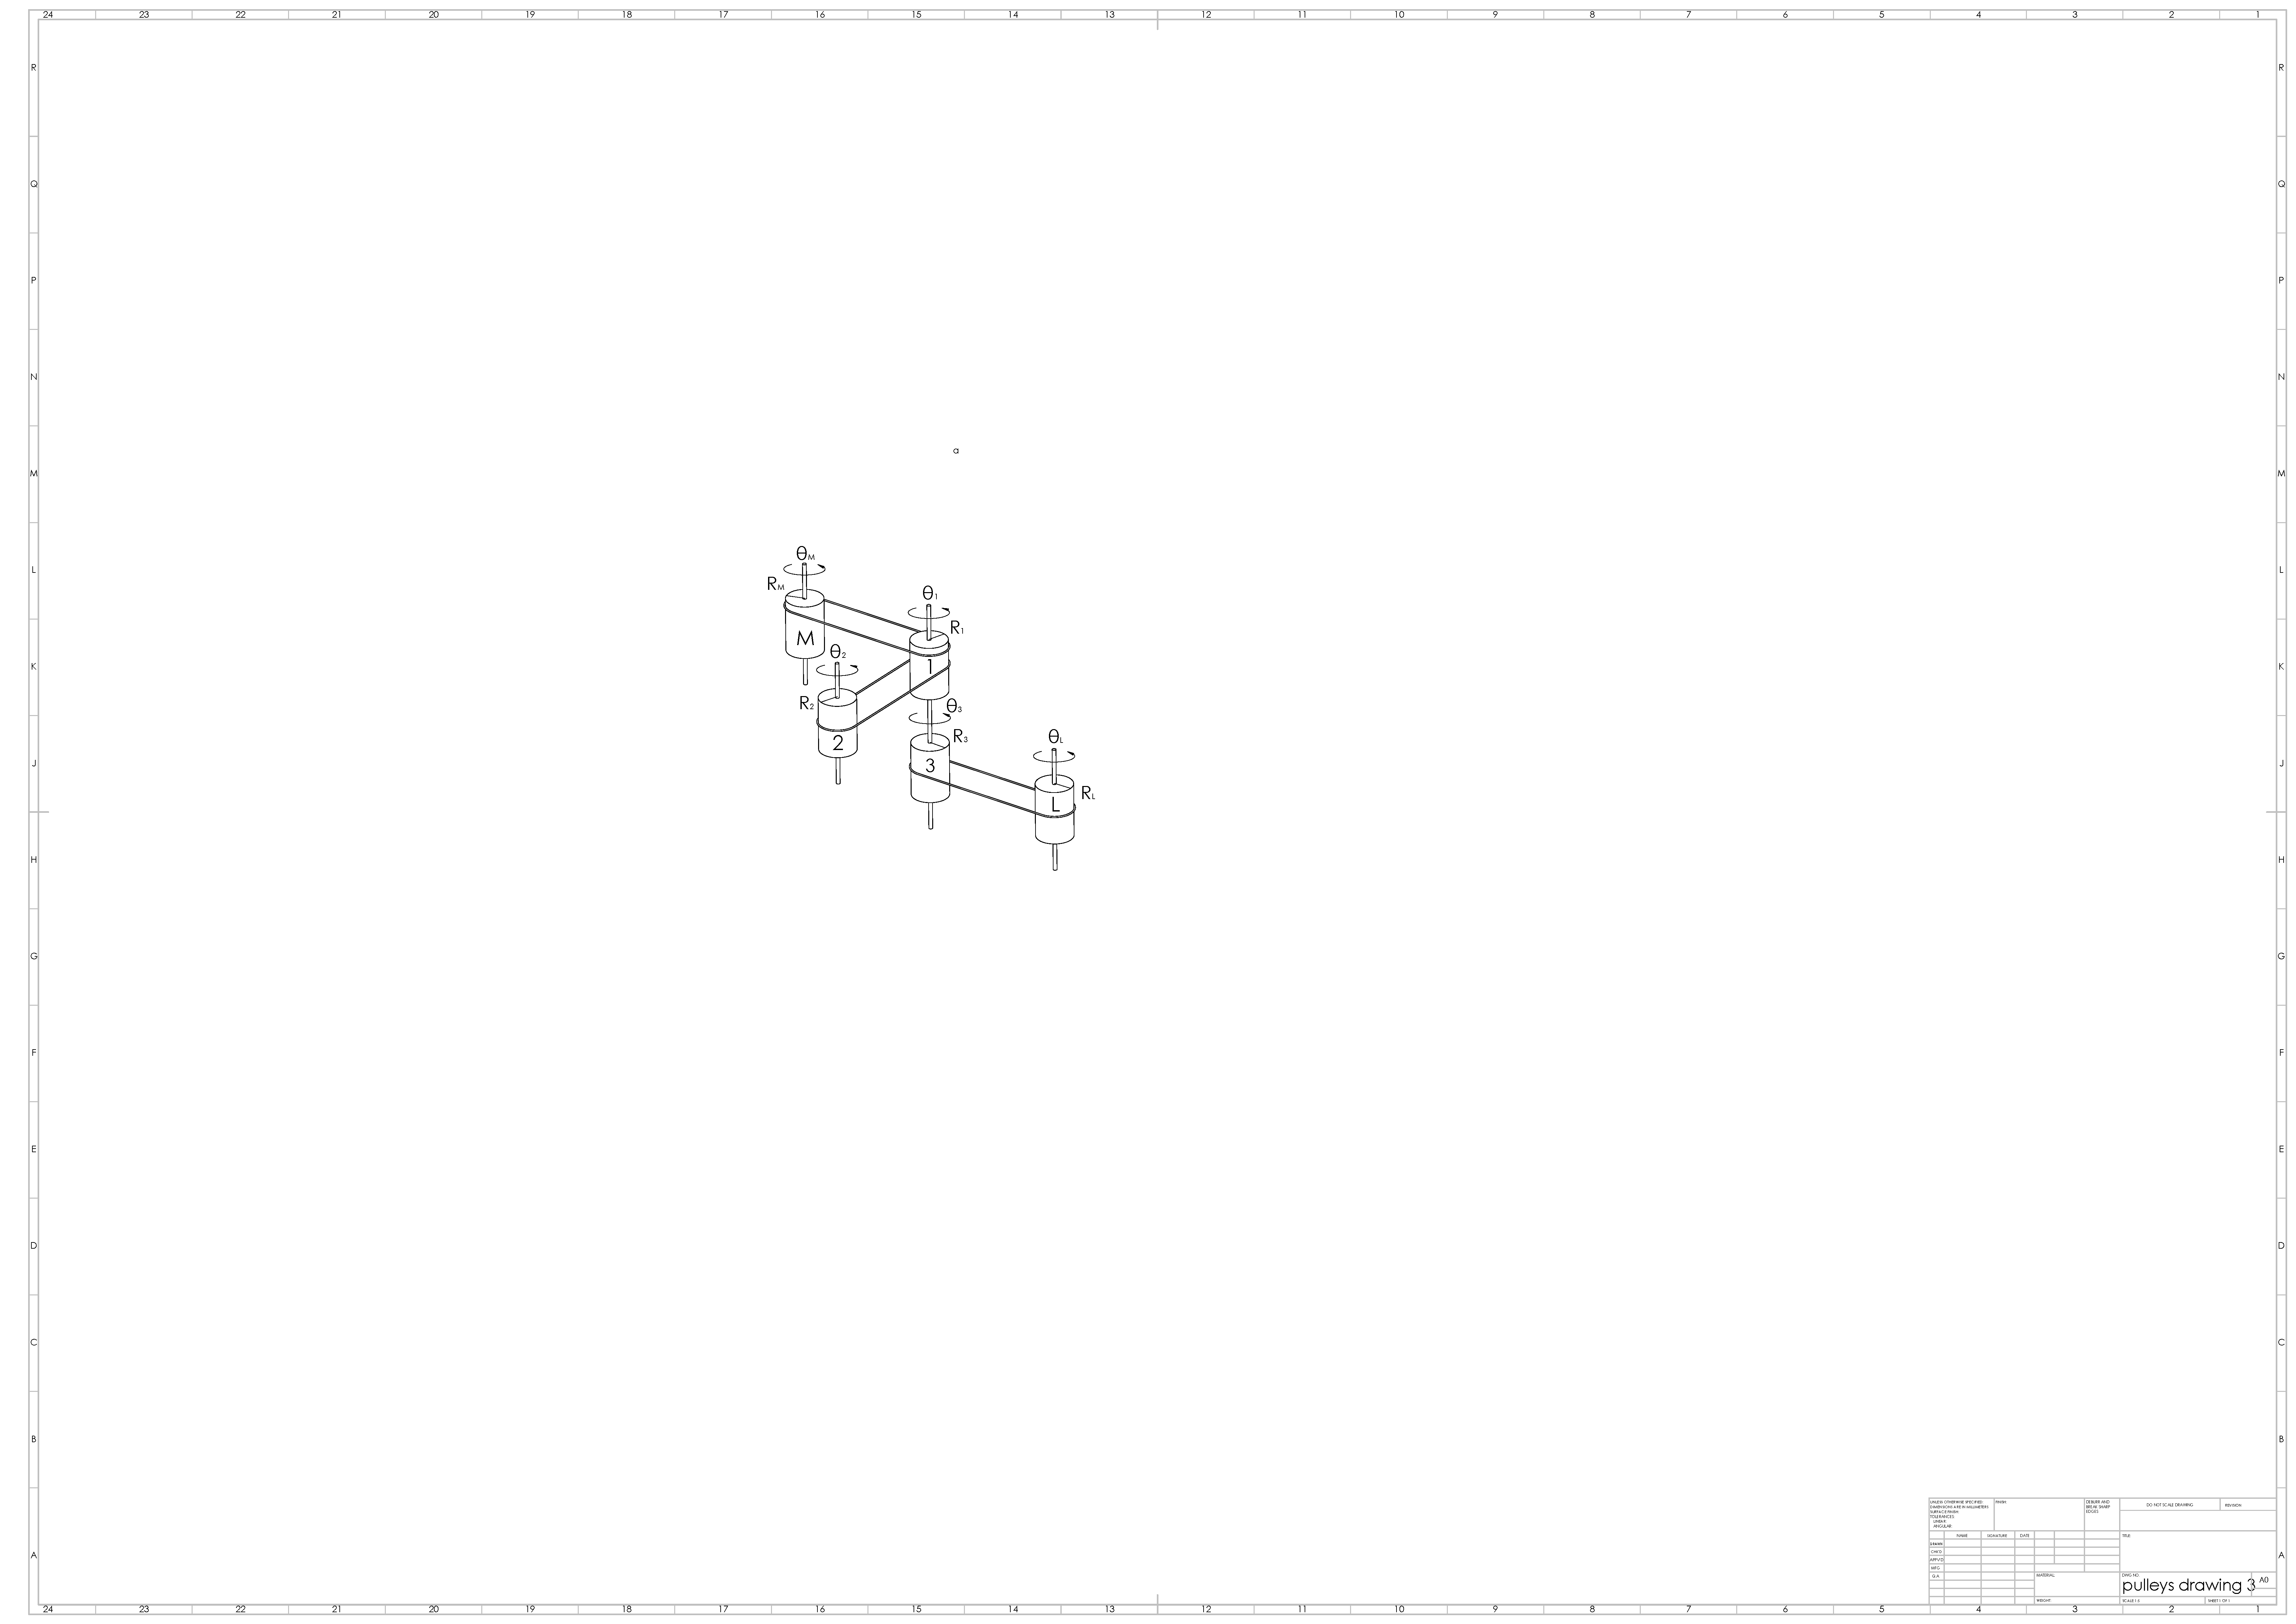
\includegraphics[width=\linewidth]{pulleys.pdf}
\caption{The pulley system of the EndoWrist gripper modeled in \cite{kim2014dynamic}.}
\label{fig:pully}
\end{figure}

The dynamical model in \cite{kim2014dynamic} is simplified to a 10th order state space system with 31 abstract, non-physical parameters, see equations \ref{sspace}-10.
This is done to simplify the process of parameter estimation.


% ATTENTION !!
% Before each equal sign include a & like this &=
% it will make the equal signs stand in a line!!
%\begin{gather}
%\begin{align}
%J_m\ddot{{\theta}_m} + B_m \dot{{\theta}_m} + R_m T_{m1}(R_m {\theta}_m - R_1 {\theta}_1) &= u_m\\
%J_L\ddot{{\theta}_L} + B_L \dot{{\theta}_L} + R_L T_{L3}(R_L {\theta}_L - R_3 {\theta}_3) &= u_L
%\end{align}
%\end{gather}


\begin{gather}\label{sspace}
\begin{align}
\dot{x}_1 &= x_2\\
\dot{x}_2 &= A_1x_1 + A_2x_2 + A_3x_3 + A_5x_5 + A_7x_7\\
\dot{x}_3 &= x_4\\
\dot{x}_4 &= B_1x_1 + B_3x_3 + B_4x_4 + B_5x_5 + B_FF\\
\dot{x}_5 &= x_6\\
\dot{x}_6 &= C_1x_1 + C_3x_3 + C_5x_5 + C_6x_6 + C_9x_9\\
\dot{x}_7 &= x_8\\
\dot{x}_8 &= K_mu_m + M_1x_1 + M_7x_7 + M_8x_8\\
\dot{x}_9 &= x_{10}\\
\dot{x}_{10} &= K_Lu_L + L_5x_5 + L_9x_9 + L_{10}x_{10}
\end{align}
\end{gather}


In equations (\ref{sspace}-10), $x_i$ represents the i-th state space vector element, while $u_L$ and $u_m$ represent the input signals for the pulley motors, see figure \ref{fig:pully}.
The resulting state vector is described in (\ref{statevector}).
\begin{align} \label{statevector}
\mathbf{x} &=
\begin{bmatrix}
\theta_1 &\dot{\theta}_1 &\theta_2 &\dot{\theta}_2 &\theta_3 &\dot{\theta}_3 &\theta_m &\dot{\theta}_m &\theta_L &\dot{\theta}_L \\
\end{bmatrix}^T
\end{align}

\subsubsection{Radial and tangential force}
Additionally, we can model the radial and tangential forces output by the yaw and roll mechanisms, respectively.

The tangential force is determined by the roll actuator and as such can be fitted to a linear model.
This is done by simple measurement with the setup in figures \ref{fig:entire_force_testsetup} and \ref{fig:endeffector_force}.

Linearity cannot be assumed for the radial output force of the yaw mechanism since it is also determined by the individual clamp actuators.
In the case where only one action is performed at any moment, the model for this force again simplifies to a (piecewise) linear one.
This assumption is confirmed experimentally as shown in figure \ref{endo_force_mes}.

\subsection{Parameter identification}
Parameter identification is performed using the Matlab parameter identification toolbox.
To tune the model’s parameters, it is necessary to perform experiments for input-output measurement datasets.

This is done by applying a known torque to the EndoWrist actuators and measuring the output force F, see figure \ref{endo_force_mes}.
The goal here is to get a fully parameterized state space model which can be used for grip, radial and tangential force estimation with a Kalman filter.

% This file was created by matlab2tikz.
%
%The latest updates can be retrieved from
%  http://www.mathworks.com/matlabcentral/fileexchange/22022-matlab2tikz-matlab2tikz
%where you can also make suggestions and rate matlab2tikz.
%
\definecolor{mycolor1}{rgb}{0.00000,0.44700,0.74100}%
\definecolor{mycolor2}{rgb}{0.85000,0.32500,0.09800}%
%
\begin{figure}[h]
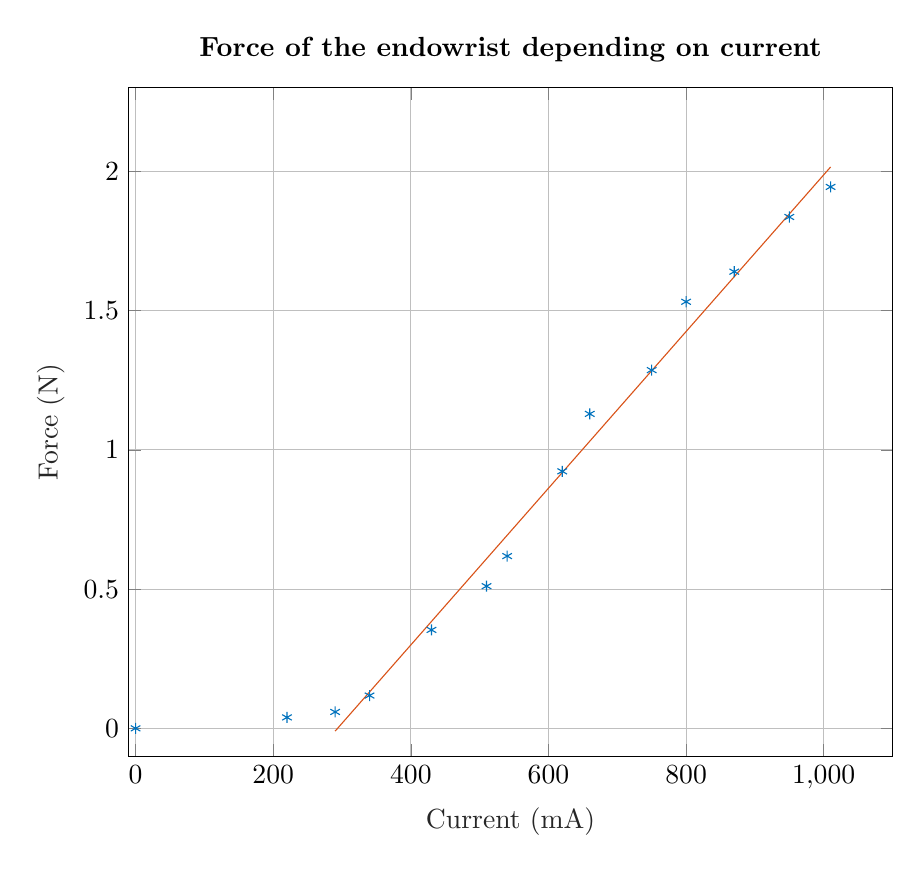
\begin{tikzpicture}

\begin{axis}[%
width=0.8\columnwidth,%7.484in,
height=0.7\columnwidth,%8.26in,
at={(0.758in,0.481in)},
scale only axis,
xmin=-10,
xmax=1100,
xlabel style={font=\color{white!15!black}},
xlabel={Current (mA)},
ymin=-0.1,
ymax=2.3,
ylabel style={font=\color{white!15!black}},
ylabel={Force (N)},
axis background/.style={fill=white},
title style={font=\bfseries},
title={Force of the endowrist depending on current},
xmajorgrids,
ymajorgrids
]
\addplot [color=mycolor1, draw=none, mark=asterisk, mark options={solid, mycolor1}, forget plot]
  table[row sep=crcr]{%
0	0\\
220	0.03928\\
290	0.05892\\
340	0.11784\\
430	0.35352\\
510	0.51064\\
540	0.61866\\
620	0.92308\\
660	1.1293\\
750	1.28642\\
800	1.53192\\
870	1.63994\\
950	1.83634\\
1010	1.94436\\
};
\addplot [color=mycolor2, forget plot]
  table[row sep=crcr]{%
290	-0.00996204344902341\\
340	0.130719594329395\\
430	0.383946542330548\\
510	0.609037162776017\\
540	0.693446145443068\\
620	0.918536765888537\\
660	1.03108207611127\\
750	1.28430902411242\\
800	1.42499066189084\\
870	1.62194495478063\\
950	1.8470355752261\\
1010	2.0158535405602\\
};
\end{axis}
\end{tikzpicture}%
\caption{The force measurements from the end-effector}
\label{endo_force_mes}
\end{figure}


At the time of writing this article, we are still in the process of developing a full setup for fitting models for grip and tangential forces.

On the other hand, the radial force model can be approximated linearly in a piecewise manner.
This is done by using a linear approximation based on input torque and output radial force measurement.


\begin{figure}
  \centering
  \begin{subfigure}{.45\linewidth}
  \vspace{30pt}
    \centering
    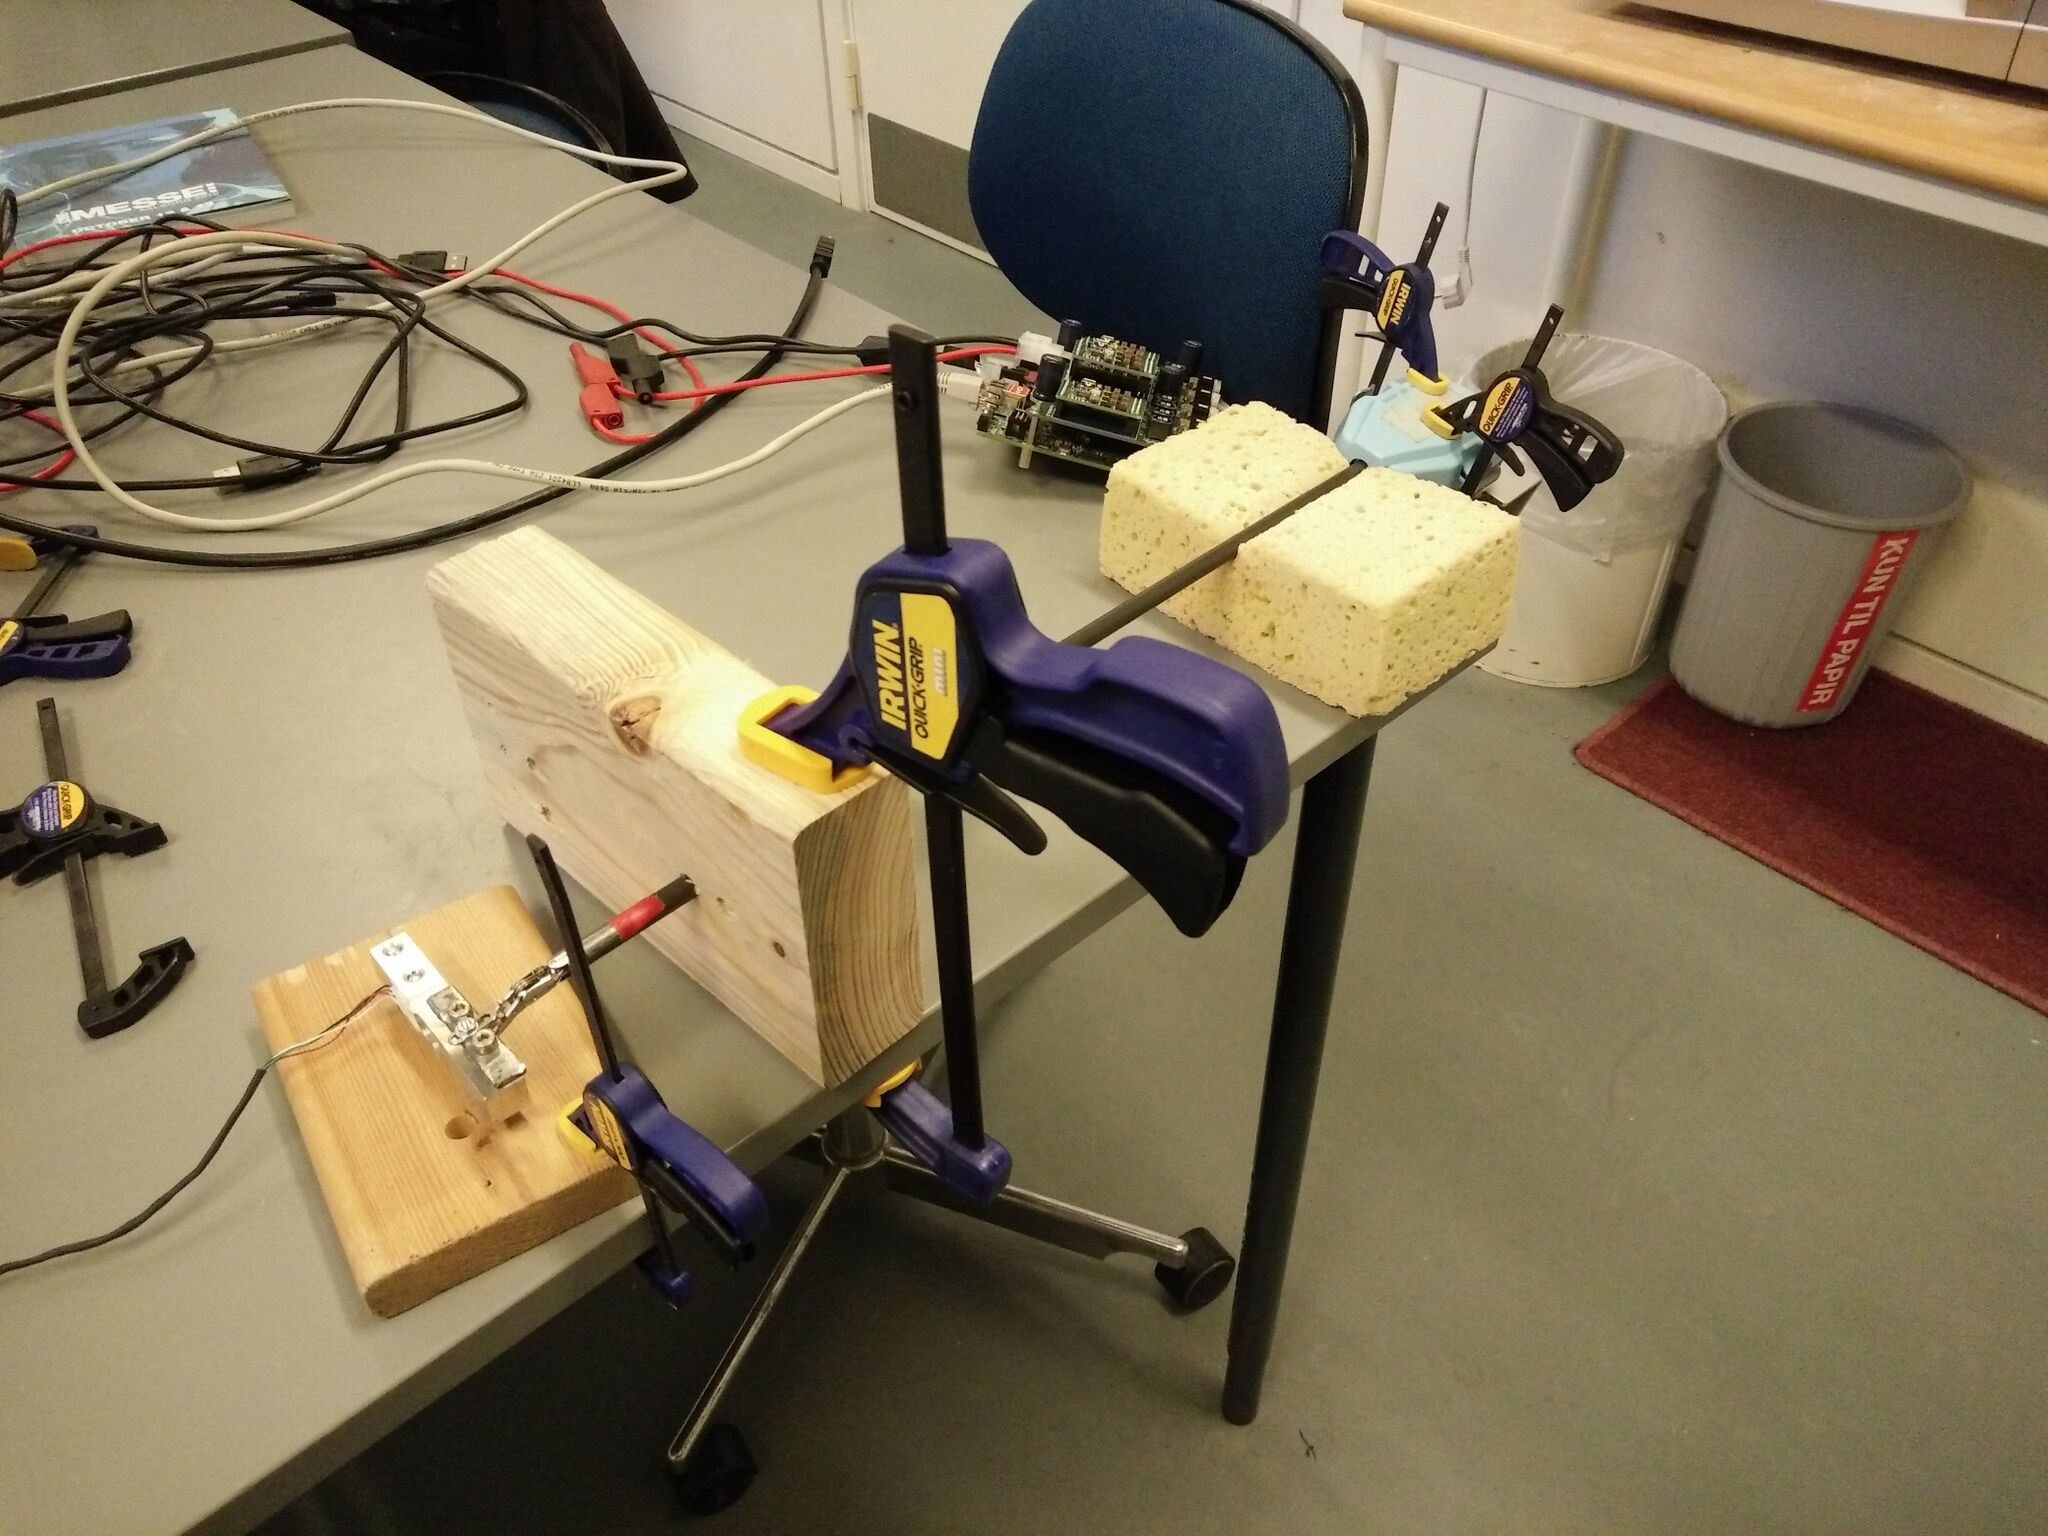
\includegraphics[width=\linewidth]{overall_force.jpg}
    \caption{The entire test setup. From the right, a scale for measuring the radial force, a piece of wood for stiffening the EndoWrist and keeping it it place and the EndoWrist holder with motors.}
    \label{fig:entire_force_testsetup}
  \end{subfigure}
  \begin{subfigure}{.45\linewidth}
    \centering
    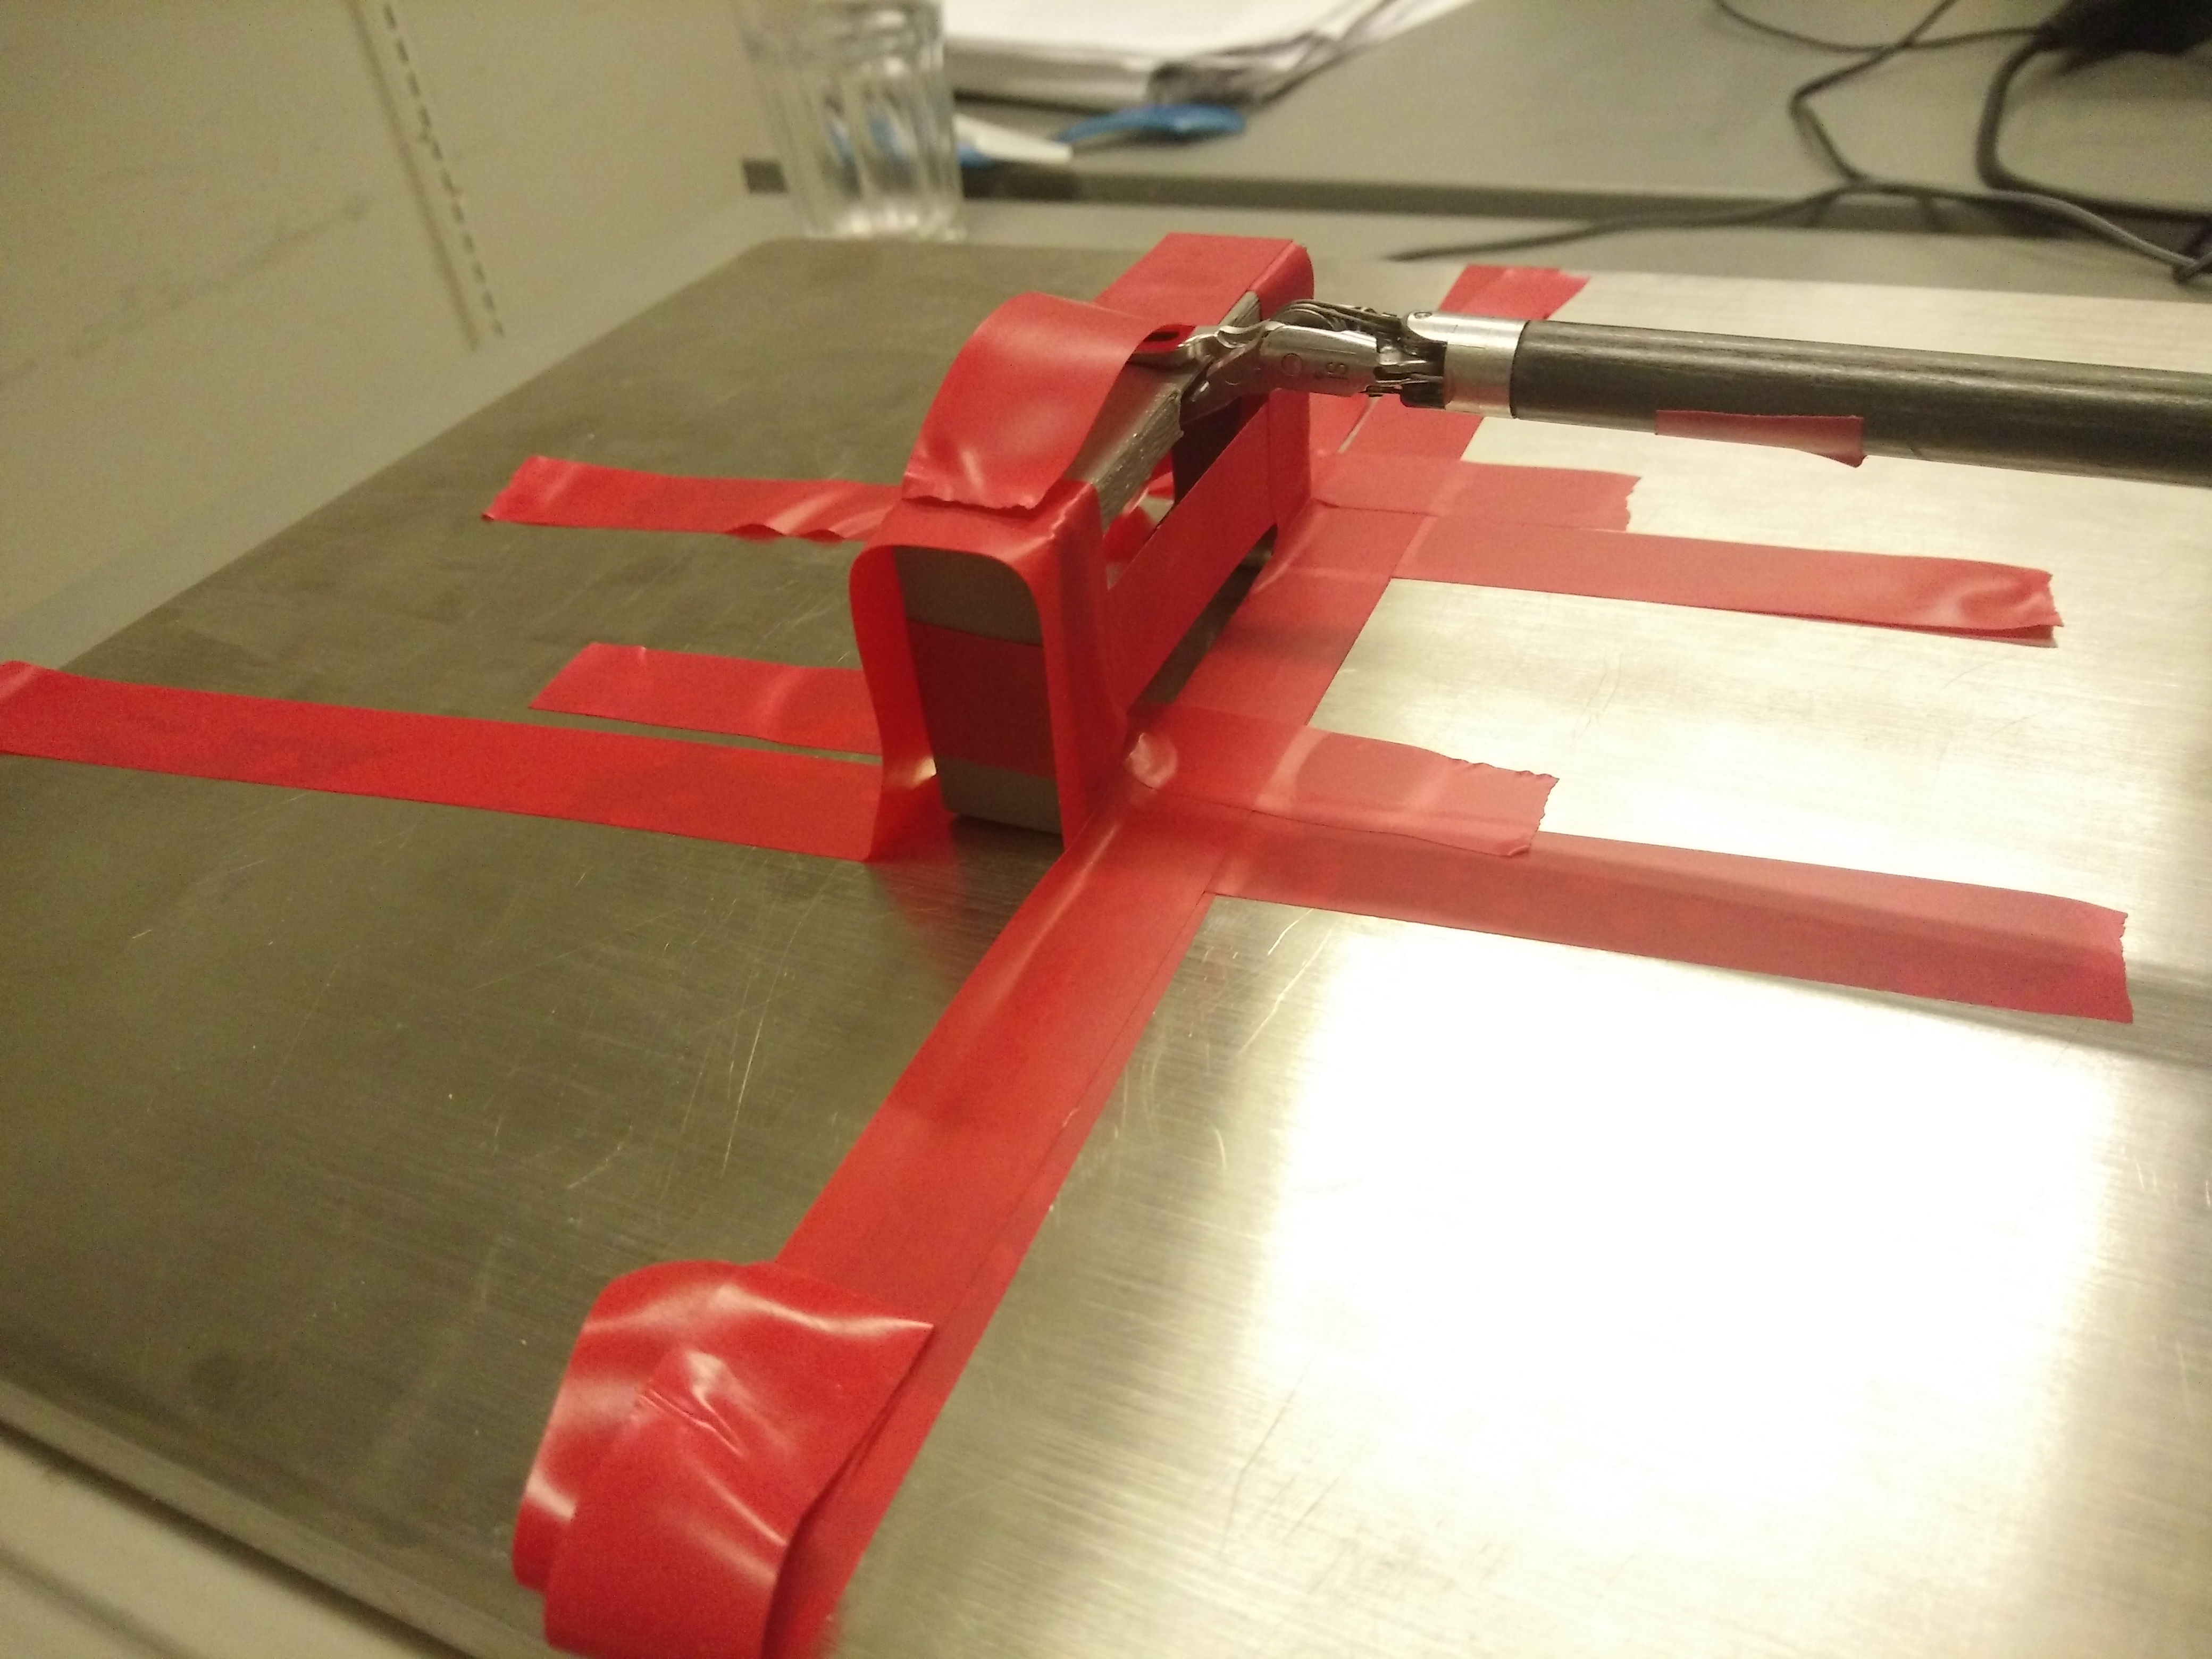
\includegraphics[width=\linewidth]{endeffector_force.jpg}
    \caption{A 3D printed case which made it possible to make an orthogonal force from the end-effector to the scale.}
    \label{fig:endeffector_force}
  \end{subfigure}
\caption{Test setup for the force estimation of the end-effector.}
\label{fig:Overview_force}
\end{figure}


A piecewise linear expression is made from the 340 mA sample and up and can be seen on equation\eqref{eq:linear_force_endo}.


\begin{equation}
F = 0.0028  \tau -0.8259
\label{eq:linear_force_endo}
\end{equation}


We consider the above equation appropriate for feedback loop implementation.
